%\documentclass[dvipdfmx,autodetect-engine,10pt,b5paper,papersize,openany]{jsbook}
\documentclass[dvipdfmx,autodetect-engine,10pt,b5paper,papersize,openany,dvipsnames]{jsbook}

\usepackage{color}
\usepackage{titlesec}
\usepackage{multicol}

% https://tex.stackexchange.com/questions/12262/multicol-and-figures
%\newenvironment{Figure}
%  {\par\medskip\noindent\minipage{\linewidth}}
%  {\endminipage\par\medskip}

% https://puarts.com/?pid=1014
\makeatletter
\newenvironment{Figure}
  {\def\@captype{figure}}
  {}
\makeatother

\usepackage{amsmath,txfonts}
\usepackage{bm}
\usepackage{mathrsfs} % \mathscr
\usepackage[dvipdfmx]{graphicx}

\usepackage{tikzpagenodes}


%\usepackage{xcolor}
\usepackage[object=vectorian]{pgfornament}
\usetikzlibrary{shapes.geometric,calc}

\usepackage{calligra}
\usepackage[T1]{fontenc}


%\usepackage[dvipdfmx]{hyperref}
\usepackage[hidelinks]{hyperref}
\usepackage{pxjahyper}

% https://oku.edu.mie-u.ac.jp/~okumura/jsclasses/
% jsbook の余白が広すぎます
% 書籍では1行の長さが全角40文字を超えないようにしています。
% そのため,段組をしないときは,自動的にどちらかの余白が広くなります
% (美文書シリーズのようなデザインになります)。
% これが困るときはプリアンブル(\begin{document} の前)に次のように書いてください。
\setlength{\textwidth}{\fullwidth}
\setlength{\evensidemargin}{\oddsidemargin}


\begin{document}


\section{Ex. 1}
例1です。

\begin{center}
  
\begin{tikzpicture}[color=Maroon,transform shape,
      %scale=1.5,
      scale=1.0,
      every node/.style={inner sep=0pt}]
  %\node[minimum size=10cm,fill=Maroon!20,inner sep=0pt](vecbox){};
  \node[minimum size=10cm,inner sep=0pt](vecbox){}; 
  \node[anchor=north west] at (vecbox.north west){\pgfornament[width=2cm]{63}};
  \node[anchor=north east] at (vecbox.north east){\pgfornament[width=2cm,symmetry=v]{63}};
  \node[anchor=south west] at (vecbox.south west){\pgfornament[width=2cm,symmetry=h]{63}};
  \node[anchor=south east] at (vecbox.south east){\pgfornament[width=2cm,symmetry=c]{63}};
  \node[anchor=north] at (vecbox.north){\pgfornament[width=6cm,symmetry=h]{46}};
  \node[anchor=south] at (vecbox.south){\pgfornament[width=6cm]{46}};
  \node[anchor=north,rotate=90] at (vecbox.west){\pgfornament[width=6cm,symmetry=h]{46}};
  \node[anchor=north,rotate=-90] at (vecbox.east){\pgfornament[width=6cm,symmetry=h]{46}};
  \node[inner sep=6pt] (text) at (vecbox.center){\Huge Ornaments};
  \node[anchor=north] at (text.south){\pgfornament[width=5cm]{75}};
  \node[anchor=south] at (text.north){\pgfornament[width=5cm,symmetry=h]{75}};
  \end{tikzpicture} 
\end{center}


\section{Ex. 2}
例2です。

\color{Maroon}
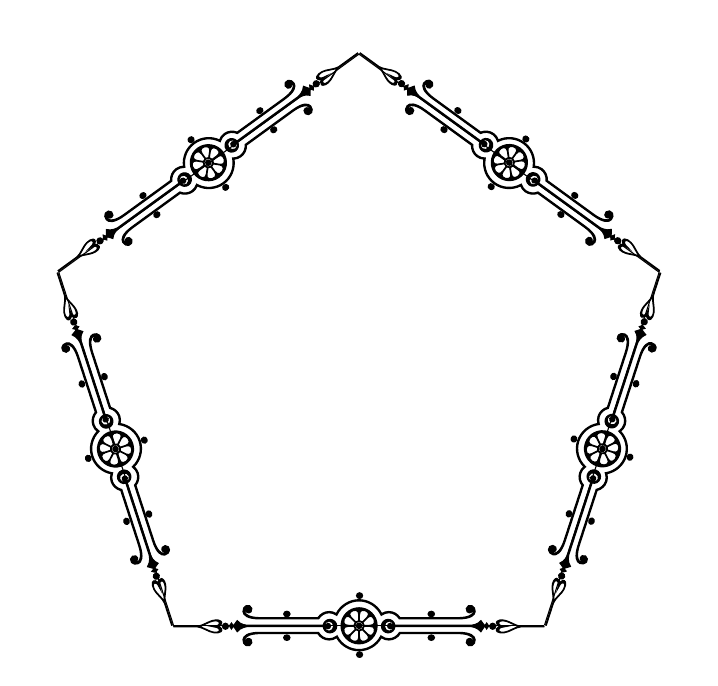
\begin{tikzpicture}
\node[regular polygon, regular polygon sides=5, 
      minimum size=8cm,inner sep=0pt](h)  {}; 
\foreach \i [count=\next from 2] in {1,...,5}
  {% 
   \draw (h.corner \i) to [ornament=84] (h.corner \next);
   \pgfmathtruncatemacro{\next}{mod(\next,5)} }
\end{tikzpicture}

\color{black}

\section{Ex. 3}
例3です。

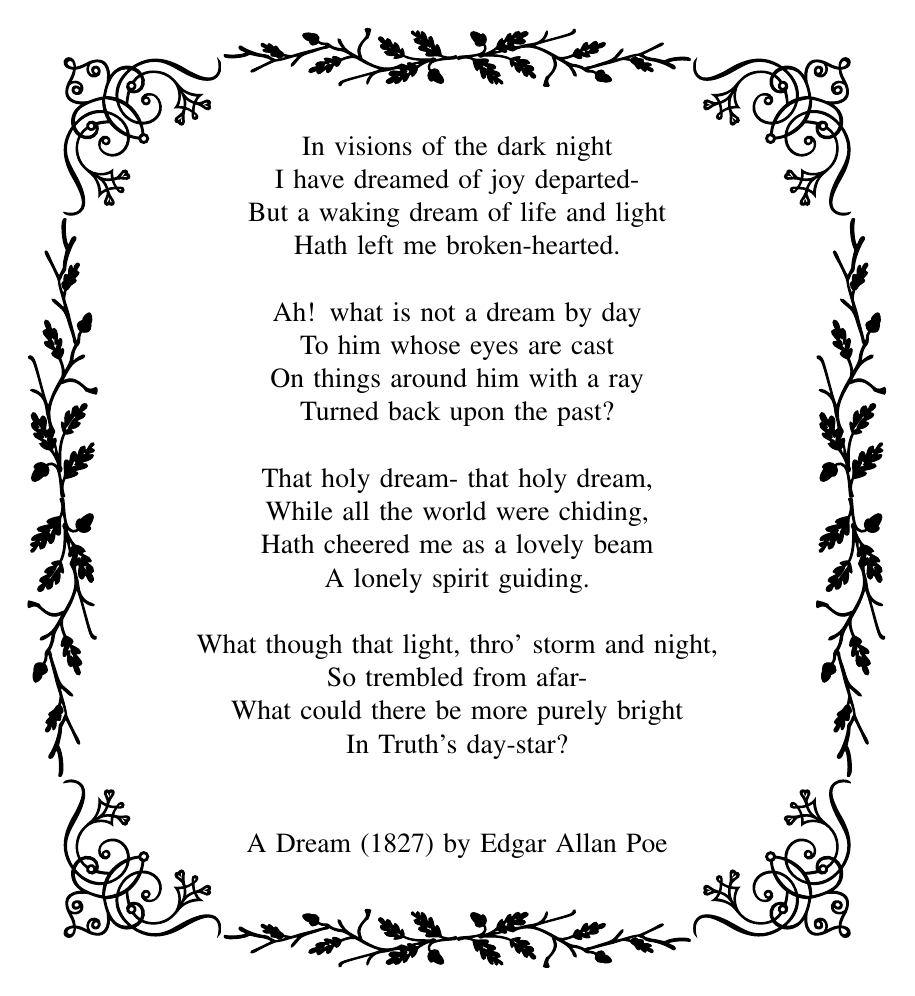
\begin{tikzpicture}[every node/.style={inner sep=0pt}]   
\node[text width=8cm,align=center](Text){%
In visions of the dark night\\
I have dreamed of joy departed-\\
But a waking dream of life and light\\
Hath left me broken-hearted.\\
\bigskip
Ah! what is not a dream by day\\
To him whose eyes are cast \\
On things around him with a ray \\
Turned back upon the past? \\
\bigskip        
That holy dream- that holy dream,\\
While all the world were chiding,\\
Hath cheered me as a lovely beam\\
A lonely spirit guiding.\\
\bigskip        
What though that light, thro' storm and night,\\
So trembled from afar- \\
What could there be more purely bright \\
In Truth's day-star? \\
\vspace{24pt}
 A Dream  (1827) by Edgar Allan Poe 
} ;
\node[shift={(-1cm,1cm)},anchor=north west](CNW)  at (Text.north west)
               {\pgfornament[width=2cm]{61}};
\node[shift={(1cm,1cm)},anchor=north east](CNE)   at (Text.north east)
               {\pgfornament[width=2cm,symmetry=v]{61}}; 
\node[shift={(-1cm,-1cm)},anchor=south west](CSW) at (Text.south west)
               {\pgfornament[width=2cm,symmetry=h]{61}}; 
\node[shift={(1cm,-1cm)},anchor=south east](CSE)  at (Text.south east)   
               {\pgfornament[width=2cm,symmetry=c]{61}};  
\pgfornamenthline{CNW}{CNE}{north}{87}
\pgfornamenthline{CSW}{CSE}{south}{87}
\pgfornamentvline{CNW}{CSW}{west}{87}
\pgfornamentvline{CNE}{CSE}{east}{87} 
\end{tikzpicture}


\section{Ex. 4}
例4です。

\setlength{\fboxsep}{0pt}
\begin{enumerate}
  \item Symmetry  vertical axis  
  \fbox{\pgfornament[width=4cm]{2}}%  
  \pgfornament[width=4cm,symmetry=v]{2} 
  
 \item Symmetry  horizontal  axis   
  \fbox{\pgfornament[width=4cm]{2}}%
  \pgfornament[width=4cm,symmetry=h]{2} 
   
 \item Origin Symmetry    
  \fbox{\pgfornament[width=4cm]{2}}% 

  \hspace*{4cm}\pgfornament[width=4cm,symmetry=c]{2}   
\end{enumerate}


\section{Ex. 5}
例5です。


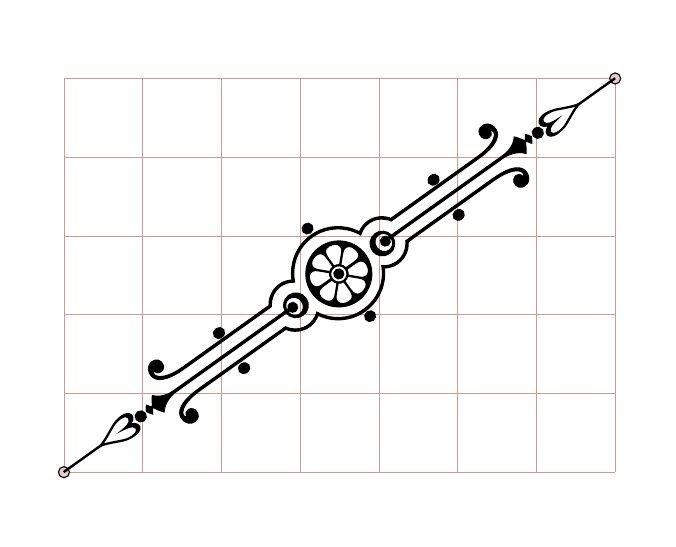
\begin{tikzpicture}
\node (A) at (0,0) {};  
\node (B) at (7,5) {}; 
\draw [help lines,color=Maroon!40]  (0,0) grid (7,5);
\draw [fill=Maroon!20]  (A) circle (2pt) (B) circle (2pt);    
\path  (A.center) to [ornament=84,
                      options/.append style={yshift=1pt}] (B.center);
\end{tikzpicture}


\section{Ex. 6}
例6です。


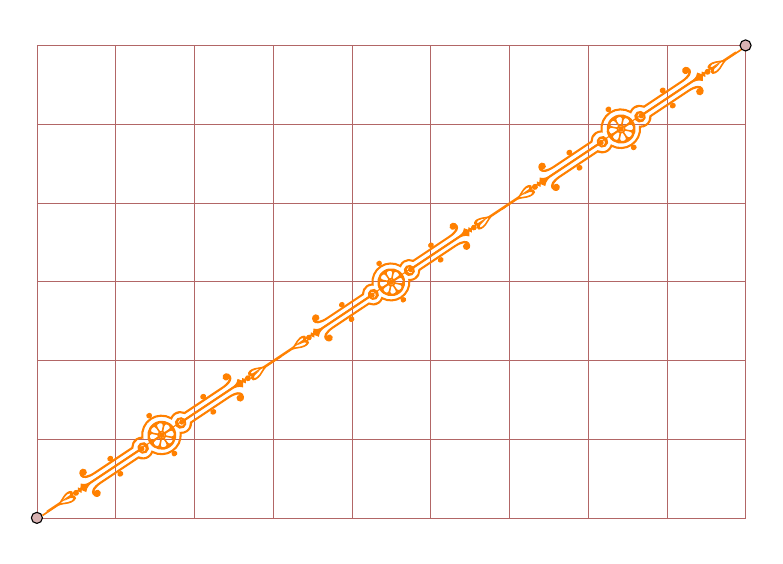
\begin{tikzpicture}
\node (A) at (0,0) {};  
\node (B) at (9,6) {}; 
\draw [help lines,color=Maroon!60]  (0,0) grid (9,6);
\draw [fill=Maroon!30]  (A) circle (2pt) (B) circle (2pt);
\path (A)--(B) coordinate[pos=.333] (c1) coordinate[pos=.666] (c2);   
\draw [orange] (A)  to [ornament=84]  (c1) to [ornament=84]  
               (c2) to [ornament=84]  (B);
\end{tikzpicture}  


\section{Ex. 7}
例7です。


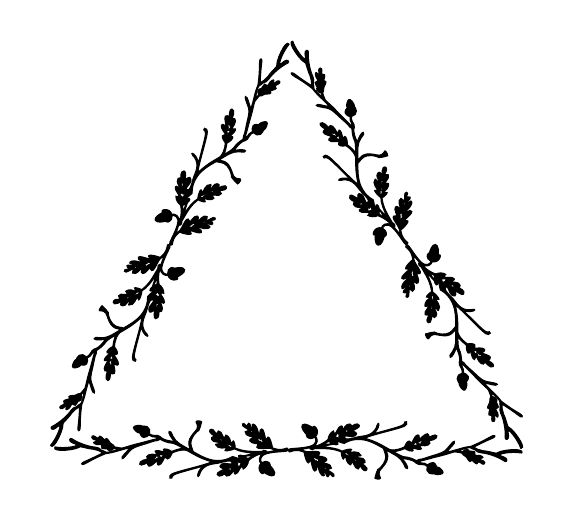
\begin{tikzpicture}
\node (A) at (0,0) {};  
\node (B) at (0:6) {};  
\node (C) at (60:6) {}; 
%\path [fill=Maroon!10,fill opacity=.4,text opacity=1]
\path
 (A.center) to [ornament=87] (B.center) to [ornament=87] 
 (C.center) to [ornament=87] (A.center);
\end{tikzpicture}


\section{網羅}
したいよね。
「89種類」と書いてある。

\begin{multicols}{3}

\begin{itemize}
  \item \# 1: \quad \pgfornament[width=3em]{1}
  \item \# 2: \quad \pgfornament[width=3em]{2}
  \item \# 3: \quad \pgfornament[width=3em]{3}
  \item \# 4: \quad \pgfornament[width=3em]{4}
  \item \# 5: \quad \pgfornament[width=3em]{5}
  \item \# 6: \quad \pgfornament[width=3em]{6}
  \item \# 7: \quad \pgfornament[width=3em]{7}
  \item \# 8: \quad \pgfornament[width=3em]{8}
  \item \# 9: \quad \pgfornament[width=3em]{9}
\end{itemize}

\begin{itemize}
  \item \# 10: \quad \pgfornament[width=3em]{10}
  \item \# 11: \quad \pgfornament[width=3em]{11}
  \item \# 12: \quad \pgfornament[width=3em]{12}
  \item \# 13: \quad \pgfornament[width=3em]{13}
  \item \# 14: \quad \pgfornament[width=3em]{14}
  \item \# 15: \quad \pgfornament[width=3em]{15}
  \item \# 16: \quad \pgfornament[width=3em]{16}
  \item \# 17: \quad \pgfornament[width=3em]{17}
  \item \# 18: \quad \pgfornament[width=3em]{18}
  \item \# 19: \quad \pgfornament[width=3em]{19}
\end{itemize}

\begin{itemize}
  \item \# 20: \quad \pgfornament[width=3em]{20}
  \item \# 21: \quad \pgfornament[width=3em]{21}
  \item \# 22: \quad \pgfornament[width=3em]{22}
  \item \# 23: \quad \pgfornament[width=3em]{23}
  \item \# 24: \quad \pgfornament[width=3em]{24}
  \item \# 25: \quad \pgfornament[width=3em]{25}
  \item \# 26: \quad \pgfornament[width=3em]{26}
  \item \# 27: \quad \pgfornament[width=3em]{27}
  \item \# 28: \quad \pgfornament[width=3em]{28}
  \item \# 29: \quad \pgfornament[width=3em]{29}
\end{itemize}

\begin{itemize}
  \item \# 30: \quad \pgfornament[width=3em]{30}
  \item \# 31: \quad \pgfornament[width=3em]{31}
  \item \# 32: \quad \pgfornament[width=3em]{32}
  \item \# 33: \quad \pgfornament[width=3em]{33}
  \item \# 34: \quad \pgfornament[width=3em]{34}
  \item \# 35: \quad \pgfornament[width=3em]{35}
  \item \# 36: \quad \pgfornament[width=3em]{36}
  \item \# 37: \quad \pgfornament[width=3em]{37}
  \item \# 38: \quad \pgfornament[width=3em]{38}
  \item \# 39: \quad \pgfornament[width=3em]{39}
\end{itemize}

\begin{itemize}
  \item \# 40: \quad \pgfornament[width=3em]{40}
  \item \# 41: \quad \pgfornament[width=3em]{41}
  \item \# 42: \quad \pgfornament[width=3em]{42}
  \item \# 43: \quad \pgfornament[width=3em]{43}
  \item \# 44: \quad \pgfornament[width=3em]{44}
\end{itemize}

\end{multicols}

\begin{multicols}{2}

\begin{itemize}

\item \# 45: \quad \pgfornament[width=0.3\textwidth]{45}
  \item \# 46: \quad \pgfornament[width=0.3\textwidth]{46}
  \item \# 47: \quad \pgfornament[width=0.3\textwidth]{47}
  \item \# 48: \quad \pgfornament[width=0.3\textwidth]{48}
  \item \# 49: \quad \pgfornament[width=0.3\textwidth]{49}
\end{itemize}

\end{multicols}

\begin{multicols}{3}

\begin{itemize}
  \item \# 50: \quad \pgfornament[width=3em]{50}
  \item \# 51: \quad \pgfornament[width=3em]{51}
  \item \# 52: \quad \pgfornament[width=3em]{52}
  \item \# 53: \quad \pgfornament[width=3em]{53}
  \item \# 54: \quad \pgfornament[width=3em]{54}
  \item \# 55: \quad \pgfornament[width=3em]{55}
  \item \# 56: \quad \pgfornament[width=3em]{56}
  \item \# 57: \quad \pgfornament[width=3em]{57}
  \item \# 58: \quad \pgfornament[width=3em]{58}
  \item \# 59: \quad \pgfornament[width=3em]{59}
\end{itemize}

\begin{itemize}
  \item \# 60: \quad \pgfornament[width=3em]{60}
  \item \# 61: \quad \pgfornament[width=3em]{61}
  \item \# 62: \quad \pgfornament[width=3em]{62}
  \item \# 63: \quad \pgfornament[width=3em]{63}
  \item \# 64: \quad \pgfornament[width=3em]{64}
  \item \# 65: \quad \pgfornament[width=3em]{65}
  \item \# 66: \quad \pgfornament[width=3em]{66}
  \item \# 67: \quad \pgfornament[width=3em]{67}
  \item \# 68: \quad \pgfornament[width=3em]{68}
  \item \# 69: \quad \pgfornament[width=3em]{69}
\end{itemize}

\end{multicols}

\begin{multicols}{2}

\begin{itemize}
  \item \# 70: \quad \pgfornament[width=0.25\textwidth]{70}
  \item \# 71: \quad \pgfornament[width=0.3\textwidth]{71}
  \item \# 72: \quad \pgfornament[width=0.25\textwidth]{72}
  \item \# 73: \quad \pgfornament[width=0.25\textwidth]{73}
  \item \# 74: \quad \pgfornament[width=0.25\textwidth]{74}
  \item \# 75: \quad \pgfornament[width=0.25\textwidth]{75}
  \item \# 76: \quad \pgfornament[width=0.25\textwidth]{76}
  \item \# 77: \quad \pgfornament[width=0.2\textwidth]{77}
  \item \# 78: \quad \pgfornament[width=0.2\textwidth]{78}
  \item \# 79: \quad \pgfornament[width=0.2\textwidth]{79}
\end{itemize}

\begin{itemize}
  \item \# 80: \quad \pgfornament[width=0.3\textwidth]{80}
  \item \# 81: \quad \pgfornament[width=0.3\textwidth]{81}
  \item \# 82: \quad \pgfornament[width=0.3\textwidth]{82}
  \item \# 83: \quad \pgfornament[width=0.3\textwidth]{83}
  \item \# 84: \quad \pgfornament[width=0.3\textwidth]{84}
  \item \# 85: \quad \pgfornament[width=0.3\textwidth]{85}
  \item \# 86: \quad \pgfornament[width=0.3\textwidth]{86}
  \item \# 87: \quad \pgfornament[width=0.3\textwidth]{87}
  \item \# 88: \quad \pgfornament[width=0.3\textwidth]{88}
  \item \# 89: \quad \pgfornament[width=0.3\textwidth]{89}
\end{itemize}

\end{multicols}

\begin{multicols}{3}


\begin{itemize}
\item \# 90: \quad \pgfornament[width=3em]{90}
\item \# 91: \quad \pgfornament[width=3em]{91}
\item \# 92: \quad \pgfornament[width=3em]{92}
\item \# 93: \quad \pgfornament[width=3em]{93}
\item \# 94: \quad \pgfornament[width=3em]{94}
\item \# 95: \quad \pgfornament[width=3em]{95}
\item \# 96: \quad \pgfornament[width=3em]{96}
\item \# 97: \quad \pgfornament[width=3em]{97}
\item \# 98: \quad \pgfornament[width=3em]{98}
\item \# 99: \quad \pgfornament[width=3em]{99}
\end{itemize}

\begin{itemize}
\item \# 100: \quad \pgfornament[width=3em]{100}
\item \# 101: \quad \pgfornament[width=3em]{101}
\item \# 102: \quad \pgfornament[width=3em]{102}
\item \# 103: \quad \pgfornament[width=3em]{103}
\item \# 104: \quad \pgfornament[width=3em]{104}
\item \# 105: \quad \pgfornament[width=3em]{105}
\item \# 106: \quad \pgfornament[width=3em]{106}
\item \# 107: \quad \pgfornament[width=3em]{107}
\item \# 108: \quad \pgfornament[width=3em]{108}
\item \# 109: \quad \pgfornament[width=3em]{109}
\end{itemize}

\begin{itemize}
\item \# 110: \quad \pgfornament[width=3em]{110}
\item \# 111: \quad \pgfornament[width=3em]{111}
\item \# 112: \quad \pgfornament[width=3em]{112}
\item \# 113: \quad \pgfornament[width=3em]{113}
\item \# 114: \quad \pgfornament[width=3em]{114}
\item \# 115: \quad \pgfornament[width=3em]{115}
\item \# 116: \quad \pgfornament[width=3em]{116}
\item \# 117: \quad \pgfornament[width=3em]{117}
\item \# 118: \quad \pgfornament[width=3em]{118}
\item \# 119: \quad \pgfornament[width=3em]{119}
\end{itemize}


\begin{itemize}
\item \# 120: \quad \pgfornament[width=3em]{120}
\item \# 121: \quad \pgfornament[width=3em]{121}
\item \# 122: \quad \pgfornament[width=3em]{122}
\item \# 123: \quad \pgfornament[width=3em]{123}
\item \# 124: \quad \pgfornament[width=3em]{124}
\item \# 125: \quad \pgfornament[width=3em]{125}
\item \# 126: \quad \pgfornament[width=3em]{126}
\item \# 127: \quad \pgfornament[width=3em]{127}
\item \# 128: \quad \pgfornament[width=3em]{128}
\item \# 129: \quad \pgfornament[width=3em]{129}
\end{itemize}

\begin{itemize}
\item \# 130: \quad \pgfornament[width=3em]{130}
\item \# 131: \quad \pgfornament[width=3em]{131}
\item \# 132: \quad \pgfornament[width=3em]{132}
\item \# 133: \quad \pgfornament[width=3em]{133}
\item \# 134: \quad \pgfornament[width=3em]{134}
\item \# 135: \quad \pgfornament[width=3em]{135}
\item \# 136: \quad \pgfornament[width=3em]{136}
\item \# 137: \quad \pgfornament[width=3em]{137}
\item \# 138: \quad \pgfornament[width=3em]{138}
\item \# 139: \quad \pgfornament[width=3em]{139}
\end{itemize}

\begin{itemize}
\item \# 140: \quad \pgfornament[width=3em]{140}
\item \# 141: \quad \pgfornament[width=3em]{141}
\item \# 142: \quad \pgfornament[width=3em]{142}
\item \# 143: \quad \pgfornament[width=3em]{143}
\item \# 144: \quad \pgfornament[width=3em]{144}
\item \# 145: \quad \pgfornament[width=3em]{145}
\item \# 146: \quad \pgfornament[width=3em]{146}
\item \# 147: \quad \pgfornament[width=3em]{147}
\item \# 148: \quad \pgfornament[width=3em]{148}
\item \# 149: \quad \pgfornament[width=3em]{149}
\end{itemize}

\begin{itemize}
\item \# 150: \quad \pgfornament[width=3em]{150}
\item \# 151: \quad \pgfornament[width=3em]{151}
\item \# 152: \quad \pgfornament[width=3em]{152}
\item \# 153: \quad \pgfornament[width=3em]{153}
\item \# 154: \quad \pgfornament[width=3em]{154}
\item \# 155: \quad \pgfornament[width=3em]{155}
\item \# 156: \quad \pgfornament[width=3em]{156}
\item \# 157: \quad \pgfornament[width=3em]{157}
\item \# 158: \quad \pgfornament[width=3em]{158}
\item \# 159: \quad \pgfornament[width=3em]{159}
\end{itemize}

\begin{itemize}
\item \# 160: \quad \pgfornament[width=3em]{160}
\item \# 161: \quad \pgfornament[width=3em]{161}
\item \# 162: \quad \pgfornament[width=3em]{162}
\item \# 163: \quad \pgfornament[width=3em]{163}
\item \# 164: \quad \pgfornament[width=3em]{164}
\item \# 165: \quad \pgfornament[width=3em]{165}
\item \# 166: \quad \pgfornament[width=3em]{166}
\item \# 167: \quad \pgfornament[width=3em]{167}
\item \# 168: \quad \pgfornament[width=3em]{168}
\item \# 169: \quad \pgfornament[width=3em]{169}
\end{itemize}

\begin{itemize}
\item \# 170: \quad \pgfornament[width=3em]{170}
\item \# 171: \quad \pgfornament[width=3em]{171}
\item \# 172: \quad \pgfornament[width=3em]{172}
\item \# 173: \quad \pgfornament[width=3em]{173}
\item \# 174: \quad \pgfornament[width=3em]{174}
\item \# 175: \quad \pgfornament[width=3em]{175}
  %\item \# 176: \quad \pgfornament[width=3em]{176}
\item \# 176: (エラー出ます)
\item \# 177: \quad \pgfornament[width=3em]{177}
\item \# 178: \quad \pgfornament[width=3em]{178}
\item \# 179: \quad \pgfornament[width=3em]{179}
\end{itemize}

\begin{itemize}
\item \# 180: \quad \pgfornament[width=3em]{180}
\item \# 181: \quad \pgfornament[width=3em]{181}
\item \# 182: \quad \pgfornament[width=3em]{182}
\item \# 183: \quad \pgfornament[width=3em]{183}
\item \# 184: \quad \pgfornament[width=3em]{184}
\item \# 185: \quad \pgfornament[width=3em]{185}
\item \# 186: \quad \pgfornament[width=3em]{186}
\item \# 187: \quad \pgfornament[width=3em]{187}
\item \# 188: \quad \pgfornament[width=3em]{188}
\item \# 189: \quad \pgfornament[width=3em]{189}
\end{itemize}

\begin{itemize}
\item \# 190: \quad \pgfornament[width=3em]{190}
\item \# 191: \quad \pgfornament[width=3em]{191}
\item \# 192: \quad \pgfornament[width=3em]{192}
\item \# 193: \quad \pgfornament[width=3em]{193}
\item \# 194: \quad \pgfornament[width=3em]{194}
\item \# 195: \quad \pgfornament[width=3em]{195}
\item \# 196: \quad \pgfornament[width=3em]{196}
\end{itemize}

\end{multicols}

以上です。


\section{創作}
してみましょう。ベースは「例1」。

テキスト変え

\begin{center}
  \begin{tikzpicture}[transform shape, scale=0.5,
      every node/.style={inner sep=0pt}]
  \node[minimum size=10cm,inner sep=0pt](vecbox){}; 
  \node[anchor=north west] at (vecbox.north west){\pgfornament[width=2cm]{63}};
  \node[anchor=north east] at (vecbox.north east){\pgfornament[width=2cm,symmetry=v]{63}};
  \node[anchor=south west] at (vecbox.south west){\pgfornament[width=2cm,symmetry=h]{63}};
  \node[anchor=south east] at (vecbox.south east){\pgfornament[width=2cm,symmetry=c]{63}};
  \node[anchor=north] at (vecbox.north){\pgfornament[width=6cm,symmetry=h]{46}};
  \node[anchor=south] at (vecbox.south){\pgfornament[width=6cm]{46}};
  \node[anchor=north,rotate=90] at (vecbox.west){\pgfornament[width=6cm,symmetry=h]{46}};
  \node[anchor=north,rotate=-90] at (vecbox.east){\pgfornament[width=6cm,symmetry=h]{46}};
  \node[inner sep=6pt] (text) at (vecbox.center){\calligra \huge
    Zenkei AI Magazine};
  \node[anchor=north] at (text.south){\pgfornament[width=5cm]{75}};
  \node[anchor=south] at (text.north){\pgfornament[width=5cm,symmetry=h]{75}};
  \end{tikzpicture} 
\end{center}

コーナーを (\#63, \#64) から (\#61, \#62)
\begin{center}
  \begin{tikzpicture}[transform shape, scale=0.5,
      every node/.style={inner sep=0pt}]
  \node[minimum size=10cm,inner sep=0pt](vecbox){};
  % コーナー
  \node[anchor=north west] at (vecbox.north west){\pgfornament[width=2cm]{61}};
  \node[anchor=north east] at (vecbox.north east){\pgfornament[width=2cm,symmetry=v]{61}};
  \node[anchor=south west] at (vecbox.south west){\pgfornament[width=2cm,symmetry=h]{61}};
  \node[anchor=south east] at (vecbox.south east){\pgfornament[width=2cm,symmetry=c]{61}};
  % 上下
  \node[anchor=north] at (vecbox.north){\pgfornament[width=6cm,symmetry=h]{46}};
  \node[anchor=south] at (vecbox.south){\pgfornament[width=6cm]{46}};
  % 左右
  \node[anchor=north,rotate=90] at (vecbox.west){\pgfornament[width=6cm,symmetry=h]{46}};
  \node[anchor=north,rotate=-90] at (vecbox.east){\pgfornament[width=6cm,symmetry=h]{46}};
  \node[inner sep=6pt] (text) at (vecbox.center){\calligra \huge
    Zenkei AI Magazine};
  \node[anchor=north] at (text.south){\pgfornament[width=5cm]{75}};
  \node[anchor=south] at (text.north){\pgfornament[width=5cm,symmetry=h]{75}};
  \end{tikzpicture} 
\end{center}



\begin{tikzpicture}
\node[regular polygon, regular polygon sides=7, 
      minimum size=8cm,inner sep=0pt](h)  {}; 
\foreach \i [count=\next from 2] in {1,...,7}
  {% 
   \draw (h.corner \i) to [ornament=81] (h.corner \next);
   \pgfmathtruncatemacro{\next}{mod(\next,7)}%
  }
  \node[inner sep=6pt] (text) at (h.center){\calligra \Large
    Zenkei\\ AI\\ Magazine};
\end{tikzpicture}



\end{document}
